\documentclass[border=12pt]{standalone}
\usepackage{tikz}
\usetikzlibrary{shapes.geometric, arrows.meta, positioning, calc, fit, backgrounds}
\usepackage{fontspec}
\usepackage{amsmath,amssymb}
\setmainfont{DejaVu Sans}

\begin{document}
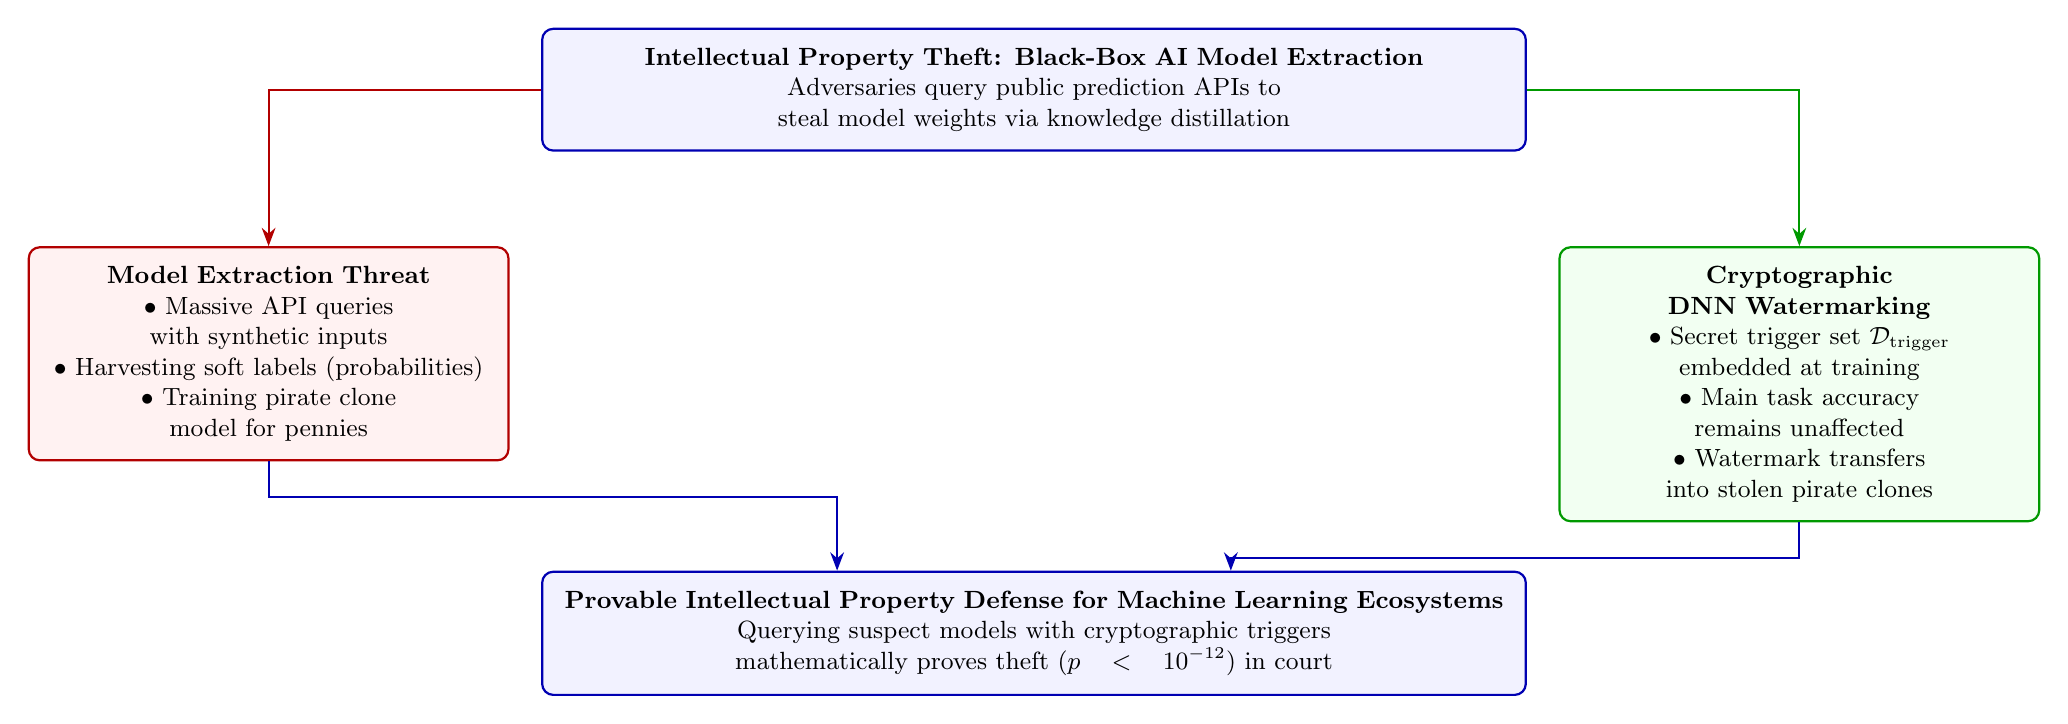
\begin{tikzpicture}[
    font=\small,
    >=Stealth,
    node distance=1.2cm,
    block/.style={rectangle, draw=blue!70!black, fill=blue!5, rounded corners=4pt, thick, align=center, inner sep=7pt},
    alertblock/.style={rectangle, draw=red!70!black, fill=red!5, rounded corners=4pt, thick, align=center, inner sep=7pt},
    greenblock/.style={rectangle, draw=green!60!black, fill=green!5, rounded corners=4pt, thick, align=center, inner sep=7pt},
    amberblock/.style={rectangle, draw=orange!80!black, fill=orange!5, rounded corners=4pt, thick, align=center, inner sep=7pt}
]

\node[block, text width=12cm] (top) {\textbf{Intellectual Property Theft: Black-Box AI Model Extraction}\\Adversaries query public prediction APIs to steal model weights via knowledge distillation};

\node[alertblock, below left=1.2cm and 0.4cm of top, text width=5.6cm] (extraction) {\textbf{Model Extraction Threat}\\$\bullet$ Massive API queries with synthetic inputs\\$\bullet$ Harvesting soft labels (probabilities)\\$\bullet$ Training pirate clone model for pennies};

\node[greenblock, below right=1.2cm and 0.4cm of top, text width=5.6cm] (watermark) {\textbf{Cryptographic DNN Watermarking}\\$\bullet$ Secret trigger set $\mathcal{D}_{\text{trigger}}$ embedded at training\\$\bullet$ Main task accuracy remains unaffected\\$\bullet$ Watermark transfers into stolen pirate clones};

\node[block, below=1.0cm of $(extraction.south)!0.5!(watermark.south)$, text width=12cm] (bottom) {\textbf{Provable Intellectual Property Defense for Machine Learning Ecosystems}\\Querying suspect models with cryptographic triggers mathematically proves theft ($p < 10^{-12}$) in court};

\draw[->, thick, red!70!black] (top) -| (extraction);
\draw[->, thick, green!60!black] (top) -| (watermark);
\draw[->, thick, blue!70!black] (extraction.south) -- ++(0,-0.45) -| ([xshift=-2.5cm]bottom.north);
\draw[->, thick, blue!70!black] (watermark.south) -- ++(0,-0.45) -| ([xshift=2.5cm]bottom.north);

\end{tikzpicture}
\end{document}
